% Options for packages loaded elsewhere
\PassOptionsToPackage{unicode}{hyperref}
\PassOptionsToPackage{hyphens}{url}
%
\documentclass[10pt,a4paper]{article}
\usepackage[left=25mm,right=25mm]{geometry}
\usepackage{amsmath}
\usepackage{amsfonts}
\usepackage{amssymb}

\usepackage{amsmath,amssymb}
\usepackage{lmodern}
\usepackage{iftex}
\ifPDFTeX
  \usepackage[T1]{fontenc}
  \usepackage[utf8]{inputenc}
  \usepackage{textcomp} % provide euro and other symbols
\else % if luatex or xetex
  \usepackage{unicode-math}
  \defaultfontfeatures{Scale=MatchLowercase}
  \defaultfontfeatures[\rmfamily]{Ligatures=TeX,Scale=1}
\fi
% Use upquote if available, for straight quotes in verbatim environments
\IfFileExists{upquote.sty}{\usepackage{upquote}}{}
\IfFileExists{microtype.sty}{% use microtype if available
  \usepackage[]{microtype}
  \UseMicrotypeSet[protrusion]{basicmath} % disable protrusion for tt fonts
}{}
\makeatletter
\@ifundefined{KOMAClassName}{% if non-KOMA class
  \IfFileExists{parskip.sty}{%
    \usepackage{parskip}
  }{% else
    \setlength{\parindent}{0pt}
    \setlength{\parskip}{6pt plus 2pt minus 1pt}}
}{% if KOMA class
  \KOMAoptions{parskip=half}}
\makeatother
\usepackage{xcolor}
\usepackage{longtable,booktabs,array}
\usepackage{multirow}
\usepackage{calc} % for calculating minipage widths
% Correct order of tables after \paragraph or \subparagraph
\usepackage{etoolbox}
\makeatletter
\patchcmd\longtable{\par}{\if@noskipsec\mbox{}\fi\par}{}{}
\makeatother
% Allow footnotes in longtable head/foot
\IfFileExists{footnotehyper.sty}{\usepackage{footnotehyper}}{\usepackage{footnote}}
\makesavenoteenv{longtable}
\usepackage{graphicx}
\makeatletter
\def\maxwidth{\ifdim\Gin@nat@width>\linewidth\linewidth\else\Gin@nat@width\fi}
\def\maxheight{\ifdim\Gin@nat@height>\textheight\textheight\else\Gin@nat@height\fi}
\makeatother
% Scale images if necessary, so that they will not overflow the page
% margins by default, and it is still possible to overwrite the defaults
% using explicit options in \includegraphics[width, height, ...]{}
\setkeys{Gin}{width=\maxwidth,height=\maxheight,keepaspectratio}
% Set default figure placement to htbp
\makeatletter
\def\fps@figure{htbp}
\makeatother
\setlength{\emergencystretch}{3em} % prevent overfull lines
\providecommand{\tightlist}{%
  \setlength{\itemsep}{0pt}\setlength{\parskip}{0pt}}
\setcounter{secnumdepth}{-\maxdimen} % remove section numbering
\ifLuaTeX
  \usepackage{selnolig}  % disable illegal ligatures
\fi
\IfFileExists{bookmark.sty}{\usepackage{bookmark}}{\usepackage{hyperref}}
\IfFileExists{xurl.sty}{\usepackage{xurl}}{} % add URL line breaks if available
\urlstyle{same} % disable monospaced font for URLs
\hypersetup{
  hidelinks,
  pdfcreator={LaTeX via pandoc}}

\author{}
\date{}



\usepackage{listings}
\usepackage{color}

\definecolor{dkgreen}{rgb}{0,0.6,0}
\definecolor{gray}{rgb}{0.5,0.5,0.5}
\definecolor{mauve}{rgb}{0.58,0,0.82}

\lstset{frame=tb,
  language=C,
  aboveskip=3mm,
  belowskip=3mm,
  showstringspaces=false,
  columns=flexible,
  basicstyle={\small\ttfamily},
  numbers=none,
  numberstyle=\tiny\color{gray},
  keywordstyle=\color{blue},
  commentstyle=\color{dkgreen},
  stringstyle=\color{mauve},
  breaklines=true,
  breakatwhitespace=true,
  tabsize=3
}

\usepackage{multicol}
\usepackage{graphicx}
\usepackage{epstopdf}

\AppendGraphicsExtensions{.gif}
\usepackage{chngcntr}
\counterwithin*{equation}{section}
\counterwithin*{equation}{subsection}

\usepackage{float} 

\usepackage{amsmath}
\let\oldsubsection\subsection
\renewcommand{\subsection}{%
    \setcounter{equation}{0}%
    \oldsubsection%
}

\begin{document}


\begin{flushleft}
\begin{LARGE}CPRE 488 Homework 4 Spring 2024
\end{LARGE}
\\PID Control
\\Jonathan Hess
\\\href{https://github.com/Jetsama/CPRE488/tree/main/HW4}{GitHub Page}
\end{flushleft}

\section{Problem 1}
\begin{quote}
Sensor Basics. Review the follow resources:\\

Accelerometer Intro:\\
https://web.archive.org/web/20230329223955/https://www.hobbytronics.co.uk/accelerometer-
info\\

Gyroscope Intro:\\
https://web.archive.org/web/20230220084525/http://www.hobbytronics.co.uk/gyro-info\\

Trade-offs:\\
https://web.archive.org/web/20230220083746/http://www.hobbytronics.co.uk/accelerometer-
gyro
\end{quote}


\subsection{Problem 1a}\begin{quote}
Given a generic 3-axis accelerometer, show the math to derive the Roll and Pitch angle of the sensor.
Simplifying assumption: assume the sensor will only be rotated about a single axis (X, Y, or Z), and that
the sensor is static when the Roll or Pitch is calculated.
\end{quote}

The force of gravity is (assumed to be) constant. Because of this we can assume that at 0 tilts we would have the full g force in the negative z direction.
\begin{figure}[H]
\centering
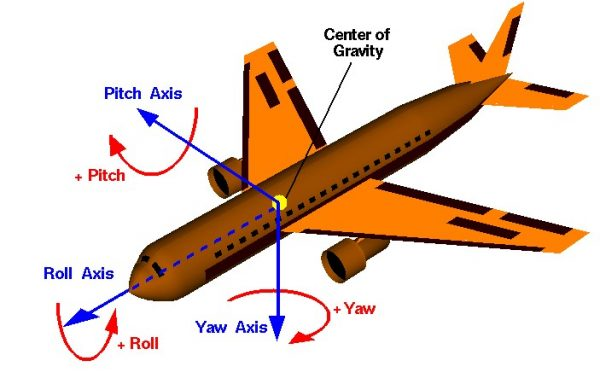
\includegraphics[width=3in]{images/rotations.jpg} \\
\caption{Rotations definitions\cite{rotation}.}
\end{figure}
\begin{figure}[H]
\centering
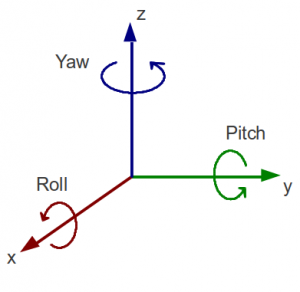
\includegraphics[width=3in]{images/rollpitchyaw.png} \\
\caption{Roll, Pitch and Yaw and XYZ axis\cite{Roll}.}
\end{figure}

To determine the Roll we can use the amount of the force has shifted to the different axis.

Using the figure we can see that the roll is determined by the X axis.\\
$Roll = sin^{-1}(x/z)$\\

This can be easily checked by using g as z and 0 as x.\\


To determine the pitch we do the same thing but with the Y axis instead.\\
$Pitch = sin^{-1}(y/z)$\\



\subsection{Problem 1b}\begin{quote}
Repeat a) for a generic 3-axis gyroscope. Simplifying assumption: assume the sensor begins at Roll,
Pitch, and Yaw orientation of (0, 0, 0) degrees, and is then rotated about a single axis to its final
orientation.
\end{quote}

The gyroscope already measures change in rotation so we can integrate that to get the current rotations.

$Roll = \int \omega_y \, dt$\\

$Pitch = \int \omega_x \, dt$\\


\section{Problem 2}
\begin{quote}
PID Control. Next, review the following resources:\\
\href{http://en.wikipedia.org/wiki/PID_controller}{Wikipedia}\\
\href{https://sites.google.com/site/fpgaandco/pid-demo}{PID-demo}\\
\end{quote}

\subsection{Problem 2a}\begin{quote}
In terms an average eighth grader could understand, explain how the P, D, and I components of a PID
controller’s correction output moves an object from an initial location to its goal location.\\
\end{quote}

There is error which is the difference between your desired value and the actual value.\\

P corrects for the current error.\\
D corrects for the average error over time.\\
I corrects for the error in the rate of change.\\

These allow to not overshoot as much when correcting for the existing error.\\


\subsection{Problem 2b}\begin{quote}
Provide pseudo-code for implementing the discrete version of the PID control algorithm.
\end{quote}

\begin{lstlisting}
PID(expected value, actual value){

last error = error;
error = expected value - actual value;
sum = sum+ error; 

u = P*error + I*(sum) + D*(error - last error);

return u

}
\end{lstlisting}


\subsection{Problem 2c}\begin{quote}
Demonstrate that you can reason about the P, I, and D components of a PID controller. In the examples
on the following page, a PID controller provides a corrective force to a ball that is being moved from
point ‘a’ to point ‘b’ on a 45 degree slope. The first plot shows the response of the ball moving from a
height of 0m to 1m under the control of a of properly tuned PID controller. For each of the remaining
plots, the P, I, and/or D constant of a PID controller has not been tuned properly. A statement has been
made for each plot. Indicate if the statement is True or False, and defend your answer.
\end{quote}


\begin{figure}[H]
\centering
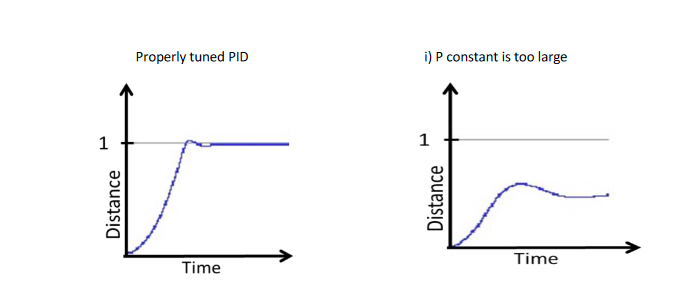
\includegraphics[width=5in]{images/Problem2-1.png} \\
\end{figure}

i) P constant is too large\\

This is false, a large P would cause the value to overshoot not undershoot. It is not correcting to the position.\\


\begin{figure}[H]
\centering
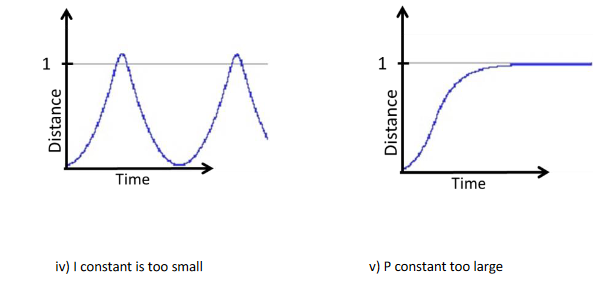
\includegraphics[width=5in]{images/Problem2-2.png} \\
\end{figure}

ii) D constant is too large\\

This is false, D constant being large would cause it to settle slower not oscillate.\\

iii) D constant is too large\\

This is true, the slow speed of change is controlled by the D.\\

\begin{figure}[H]
\centering
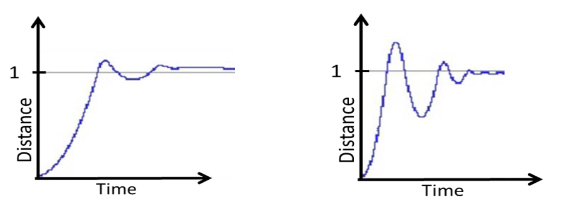
\includegraphics[width=5in]{images/Problem2-3.png} \\
\end{figure}

iv) I constant is too small \\
False, a small I value would not cause oscillation. Increasing I would only create worse oscillations.

v) P constant too large\\
This is true. The overshooting is a sign that it is underdamped and is over correcting for the positional error.
\begin{thebibliography}{9}

\bibitem{rotation}\href{https://www1.grc.nasa.gov/beginners-guide-to-aeronautics/aircraft-rotations/}{NASA: Aircraft Rotations}
\bibitem{Roll}\href{https://xmarklabs.com/blog/2017/08/mysteries-tracking/rollpitchyaw/}{Roll, Pitch and Yaw}

\end{thebibliography}

\end{document}
